\subsection{Experimental Setup}
\label{exp:setup}

\textbf{Models and system configuration.}
We conduct tests using three open-source OPT models of different scales (i.e., OPT-6.7B, OPT-13B, and OPT-30B). Our experiments are performed on a server with 2 $\times$ AMD EPYC 7763 CPUs (64 cores), 128 GB DRAM, one NVIDIA A100 GPU with 80GB HBM, and one 2TB Intel SSD whose measured read throughput is around 5GB/s. The GPU and CPU are connected via PCIe 4.0 $\times$ 16.

\noindent \textbf{Datasets and metrics.}
%We use four representative datasets covering three typical tasks involving shared prefixes: 
%(1) Few-shot tasks. We use two datasets from the lm-evaluation-harness benchmark~\cite{lmeval}: PIQA and OpenBookQA. Each request starts with two to ten examples as the few-shot prefix.
%(2) RAG-based question answering tasks. We use a reading comprehension dataset, SQuAD~\cite{squad-arxiv18}, where multiple queries are involved for the same passage prefix.
%(3) System-prompt-based tasks. Forty-five system prompts that explicitly define the functionalities of the GPT store plugins~\cite{gptsysprompt} are used as prefixes. Similar to~\cite{cacheblend-arxiv24}, we use the GPT-4 API to generate three more similar queries for each system prompt.
We select four representative datasets from the standard LM-Evaluation-Harness benchmark~\cite{lmeval}: PIQA, RTE, COPA, and OpenBookQA. 
\fv{
These datasets are designed for few-shot tasks and structured as multiple-choice questions to evaluate the capabilities of large models in commonsense reasoning, logical inference, causal reasoning, and science question answering, respectively. 
%In total, there are approximately 400 user requests for PIQA and around 1,000 requests for each of the other three datasets.
}
Due to the lack of open-source, real-world datasets for prefix reuse, we adopt a similar approach to previous work~\cite{infinigen-osdi24} by prepending two to ten few-shot examples as system prompts before each query. These system prompts are shared across different queries, with reuse frequency following a normal distribution.

%We measure model generation quality using accuracy, following the same metric employed in prior works~\cite{infinigen-osdi24, h2o-nips23}.
%We vary the user-defined prefix KV retention ratios from 50\% to 5\% to observe changes in model accuracy.
\fvc{
We measure model generation quality using accuracy, as in prior works~\cite{infinigen-osdi24, h2o-nips23}, and vary the prefix KV retention ratios from 50\% to 5\% to observe accuracy changes.
}
Additionally, to test TTFT with long prefixes as in~\cite{cachegen-sigcomm24} and to prevent runtime out-of-memory errors, we extend the prefixes to a maximum length of 4K for OPT-30B and 10K for the other OPT models.
\fv{
The average number of tokens in the request prefixes across the four datasets ranges from 4.8k to 5.7k.
}

\noindent \textbf{Baseline systems.}
We compare \pname{} with four baselines.
(1) \textit{ReComp}~\cite{alluneed-nips17}: It recomputes all prefix KVs for each request without storing or reusing them.
(2) \textit{AS-like}~\cite{attentionstore-atc24}: AttentionStore (AS)
asynchronously stores and loads all shared prefix KVs. Since it is not
open-source, we reimplement it to the best of our ability based on the paper. To
ensure a fair comparison, we additionally add the GPU cache with LRU for prefix KV
storage. Besides, we disable its scheduler-aware optimizations to make it more
suitable for general scenarios, such as preemptive scheduling environments.
(3) \textit{AS+H2O+LRU}: We combine AS-like with one of the state-of-the-art important KV selection systems, H2O~\cite{h2o-nips23}. Different from the AS-like, it asynchronously loads only important values rather than the full values of shared prefixes.
(4) \textit{AS+H2O+LFU}: It is similar to (3), but it uses LFU to manage the cache.
%We believe both (3) and (4) represent state-of-the-art systems for accelerating prefix KV loading from storage, combining existing optimization techniques.
In contrast, \pname{} selectively loads partial keys and values, 
%enables KV reordering, and employs a score-based cache management strategy.
\fvc{
reorders KVs, and uses a score-based cache management strategy.
}

% \he{By default, we allocate 10GB of GPU cache and 32GB of CPU cache to avoid runtime out-of-memory errors for all the systems.}
% The average prefix KV storage requirements for PIQA, RTE, COPA, and OpenBookQA across three models are 55 GB, 57 GB, 64 GB, and 65 GB, respectively.
% Each chunk contains 64 tokens' keys or values in all systems~\cite{chunkattention-arxiv24}.
% We clarify that in our scenario, the entire query is always retained, unlike
% existing KV pruning systems~\cite{h2o-nips23, infinigen-osdi24}.

To prevent runtime out-of-memory errors and ensure only a portion of the prefix
KVs are cached (the other KVs reside on SSD), we allocate 10GB of GPU cache and 32GB of CPU cache for prefix
KVs, leaving the remaining GPU and CPU memory for storing model weights, the KV cache
used during the decoding phase, and the input data.
%\he{By default, we assign 10GB to GPU cache and 32GB to CPU cache across all systems to prevent memory overflow.} 
On average, PIQA, RTE, COPA, and OpenBookQA require 55GB, 57GB, 64GB, and 65GB of storage for prefix KVs across three models, respectively. Uniformly, each chunk holds keys or values from 64 tokens~\cite{chunkattention-arxiv24}. 
%Note that, unlike conventional KV pruning systems~\cite{h2o-nips23, infinigen-osdi24}, we retain the full query in our scenario.

\begin{figure*}
	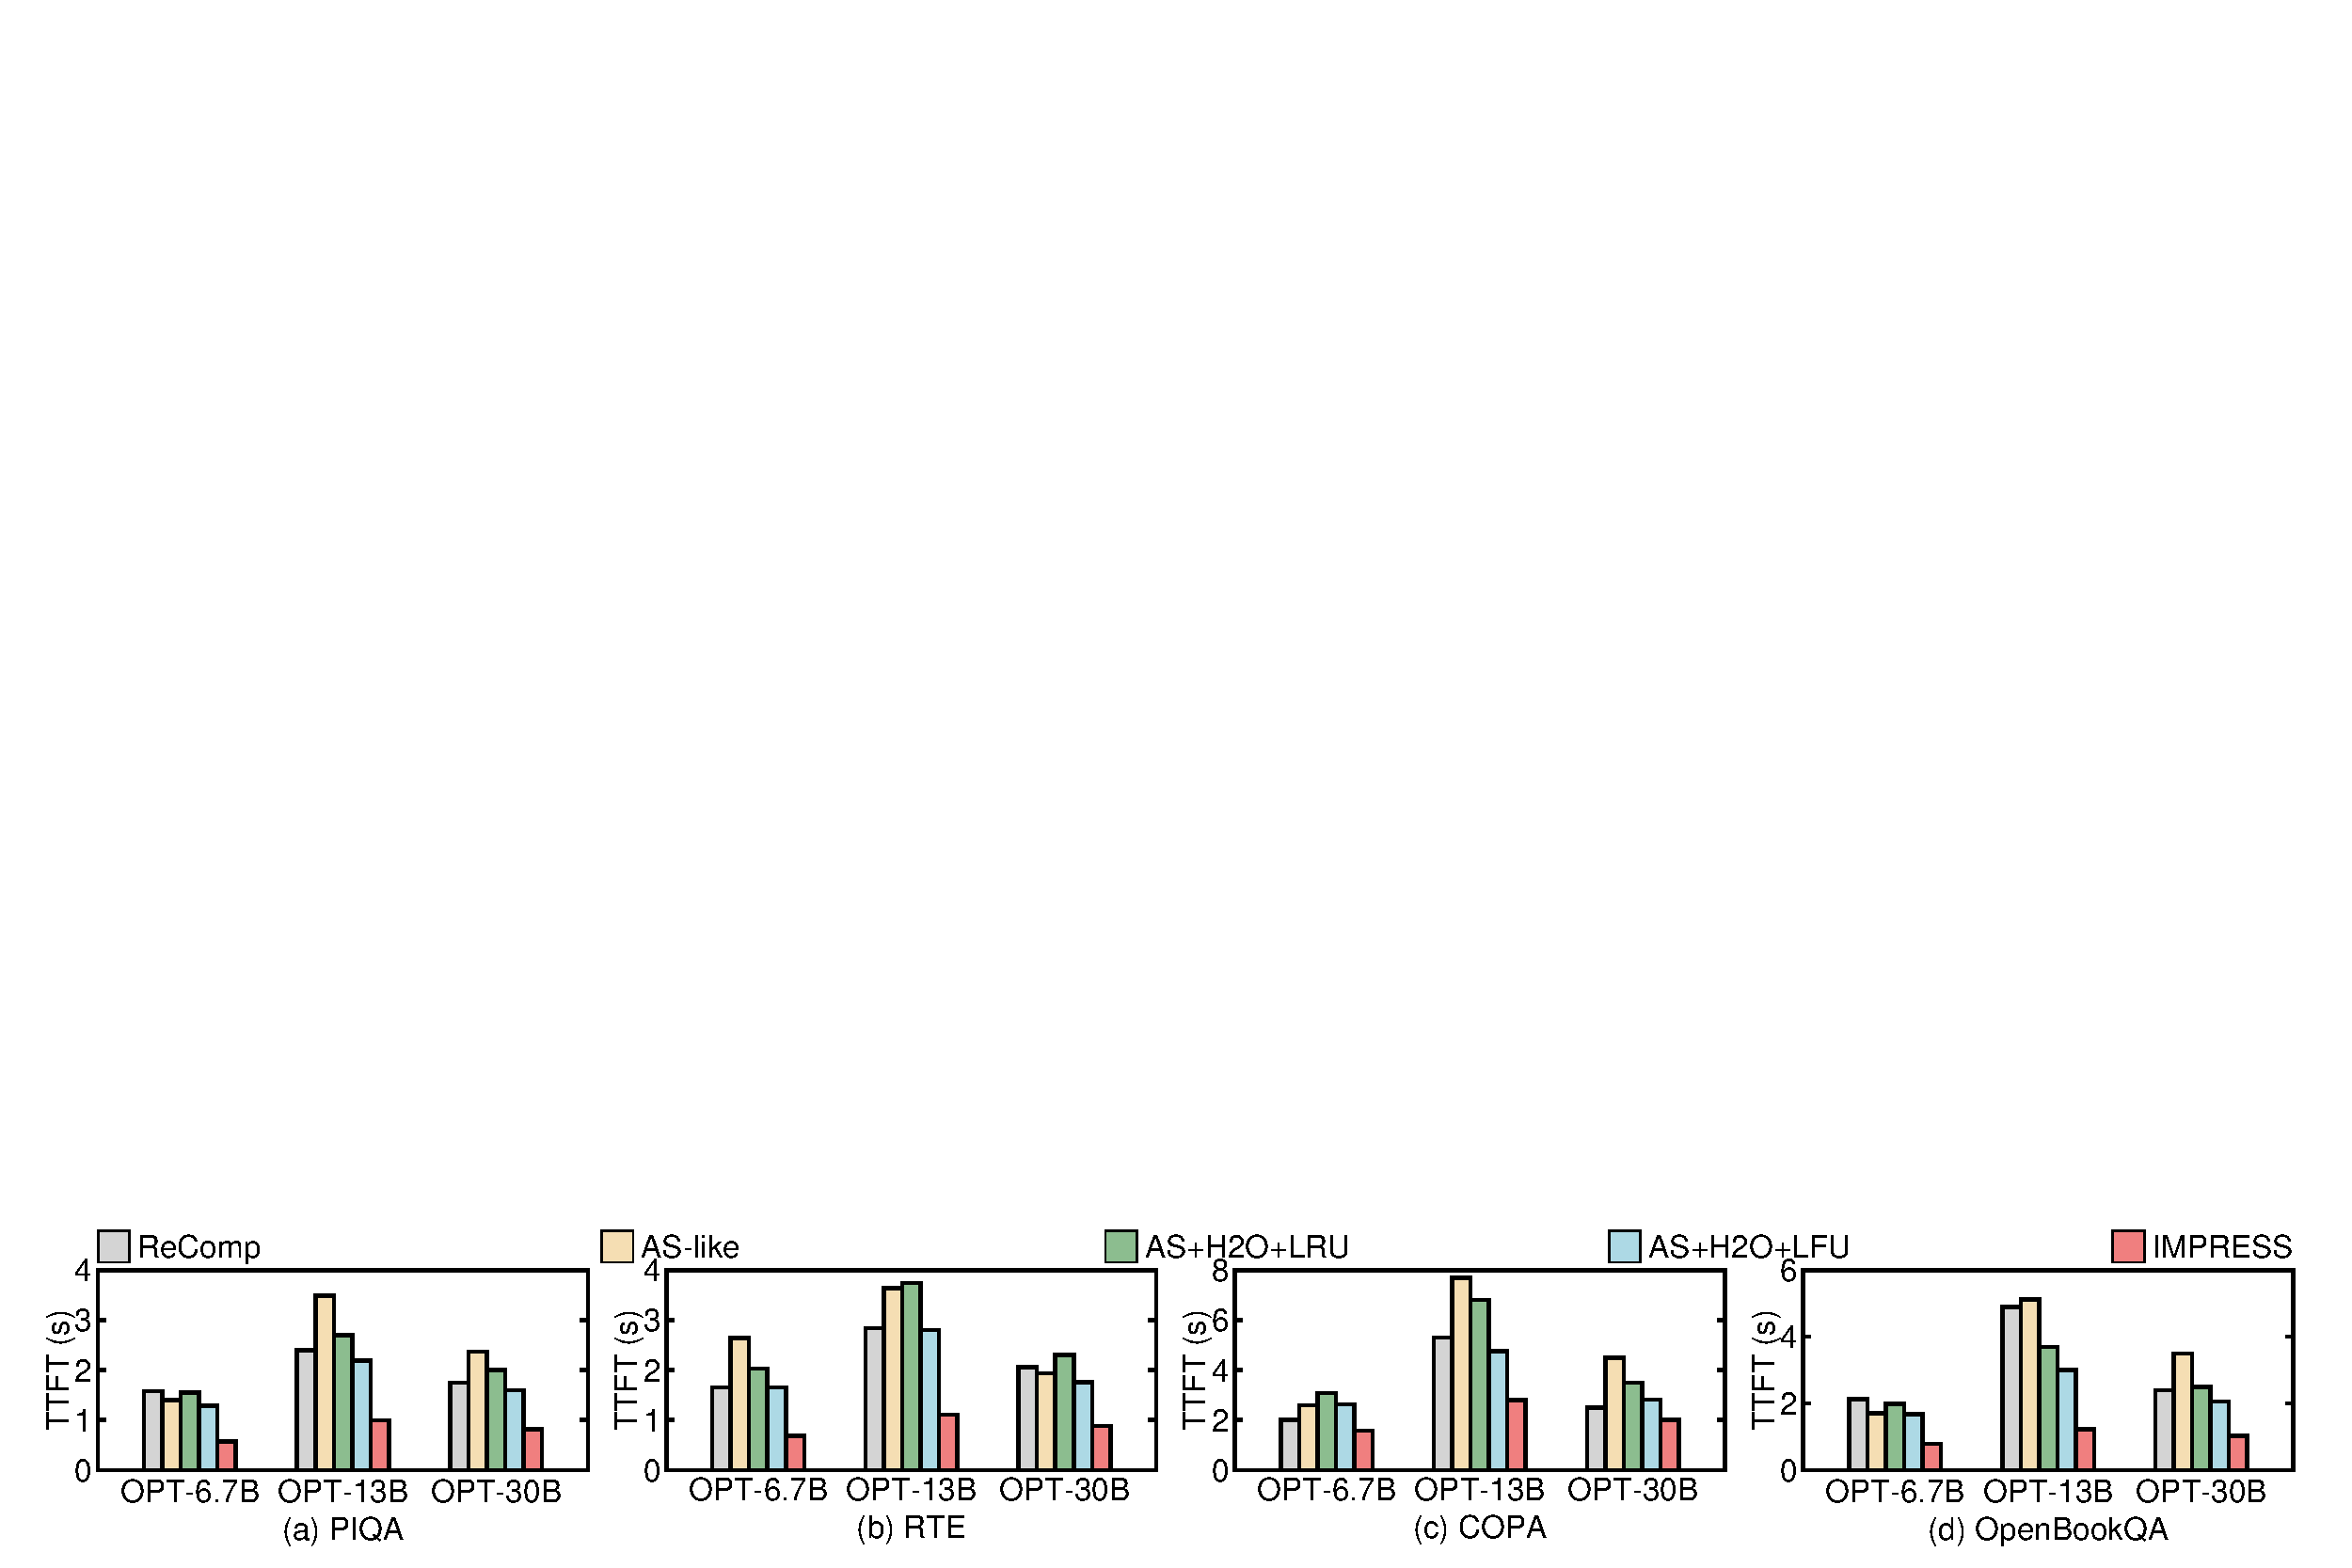
\includegraphics[width=7in, height=1in]{ttft_ds1_ds2_ds3_ds4.pdf}
	\vspace{-0.2in}
	\caption{
		The average TTFT with various systems across four dataset and three models.}
	\label{fig:overall_ttft}
	\vspace{-0.1in}
\end{figure*}